
\quad В какой-то момент при работе за виртуальной машиной, высветилось сообщение о том, что память заканчивается. 

\quad Для начала вводим в поисковике Linux-а «Диски» и, нажав на иконку диска, смотрим насколько он заполнен, и сколько памяти осталось. 

\begin{figure}[h]
		\centering
		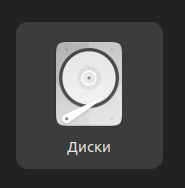
\includegraphics[width=0.3\linewidth]{VM/15.1.png}
\caption{Иконка диска.}
\label{ris:image}
\end{figure}

\quad Необходимо выключить виртуальную машину, а не сохранить, чтобы можно было изменить её настройки. Далее в меню VirtualBox выбираем пункт «Файл» и нажимаем на «Менеджер виртуальных носителей…».

\quad В открывшемся окне заходим в свойства диска и находим его размер. Двигая за ползунок, изменяем его объём с 16 гигабайт до 33 и нажимаем «Применить». 

\begin{figure}[h]
		\centering
		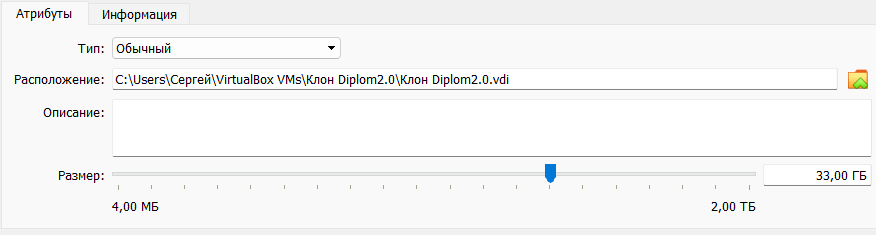
\includegraphics[width=0.7\linewidth]{VM/15.2.png}
\caption{Изменение размера диска.}
\label{ris:image}
\end{figure}

\quad При повторном открытии виртуальной машины было обнаружено, что размер памяти не изменился. Мы пришли к выводу, что для того чтобы увеличить объём памяти жёсткого диска, нужно сделать клон текущего состояния виртуальной машины или удалить снимки. К сожалению изменять размер диска, просто нельзя, пока существуют его точки сохранения. Поэтому снова выключаем машину, и делаем клон её текущего состояния. Он делается точно так же, как когда мы делали клон для переноса его с одного устройства на другое. Единственное отличие в том, что в этот раз выбираем клонировать не всё, а только текущее состояние. 

\quad Увеличив в «Менеджере виртуальных носителей…» уже объём памяти клона, заходим в настройки виртуальной машины, увеличиваем размер памяти в «Системе» и выбраем соответствующий диск в «Носителях», так же как это делали, после переноса клона на другое устройство. Далее запускаем новую машину и заходим в «Диск», где видим, что его размер стал больше, и появилась дополнительная область памяти.

\quad Чтобы задействовать его, нажимаем на иконку настроек, сдвигаем ползунок до конца вправо, чтобы можно было использовать всю новую память и нажиимаем «Применить», после чего вводим свой пароль. Но опять ничего не получилось. Чтобы наконец всё заработало, нужен установочный файл Ubuntu нашей виртуальной машины. Он остался на прошлом устройстве, с которого мы и клонировали машину. Воспользовавшись гугл диском, перенесли файл, так как флэшка не позволяет загрузить в неё что-либо весом более 4 гигабайт без её форматирования.

\quad После перенесения установочный файла на новое устройство, необходимо добавить его в настройках виртуальной машины. Для этого нажать «Настроить», зайти в «Носители», кликнуть по пустому диску, и в «Оптическом приводе» выбрать файл установки.

\begin{figure}[h]
		\centering
		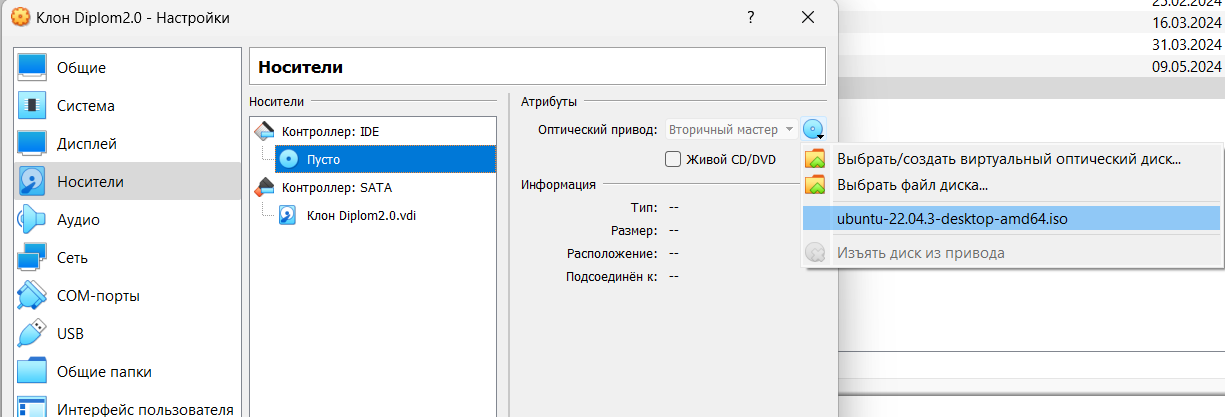
\includegraphics[width=0.9\linewidth]{VM/15.png}
\caption{Добавление установочного файла.}
\label{ris:image}
\end{figure}

\quad При запуске виртуальной машины, нужно выбрать пункт "Try or Install Ubuntu" и далее нажать "Try Ubuntu". 

\quad Необходимо так же установить приложение «GParted».
\newline \quad • Первым шагом нужно обновить списки пакетов, введя в терминале команду: «sudo apt-get update». 
\newline \quad • Далее установить «GParted» командой: «sudo apt-get install gparted». 
\newline \quad • Ввести пароль, когда это предложат. 
\newline \quad • После установки «GParted», его наконец-то можно запустить из меню приложений или с помощью команды: «sudo gparted». 

\quad В открывшемся меню нужно кликнуть правой кнопкой мыши по области «/dev/sda3» и выбрать пункт «Изменить размер/Переместить». Далее, двигая за ползунок с правого края, можно наконец позволить виртуальной машине использовать всё добавленное, свободное пространство. Снова нажимаем на кнопку «Изменить размер/Переместить». И в меню «GParted»  кликаем по зелённой галочке, чтобы применить все внесённые изменения. После недолгой загрузки закрываем «GParted».

\begin{figure}[h]
		\centering
		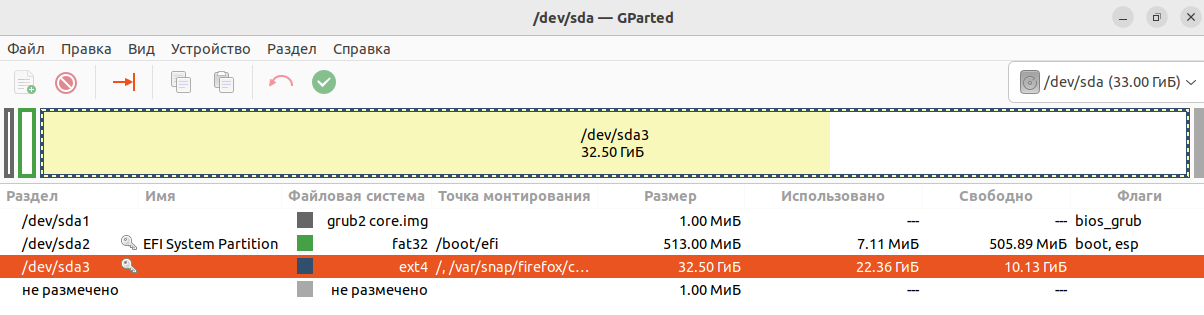
\includegraphics[width=0.9\linewidth]{VM/15.3.png}
\caption{Gparted.}
\label{ris:image}
\end{figure}

\quad Чтобы при каждом запуске виртуальной машины, установочный файл не предлагал установить «Ubuntu», нужно удалить его в настройках виртуальной машины так же, как мы его и добавляли.
